% begin module continuous-def
\begin{frame}
\frametitle{Continuity}
\begin{definition}[Continuous at a Number]
A function $f$ is continuous at a number $a$ if
\[
\lim_{x\rightarrow a}f(x) = f(a) .
\]
\end{definition}
\begin{columns}[c]
\column{.5\textwidth}
\ 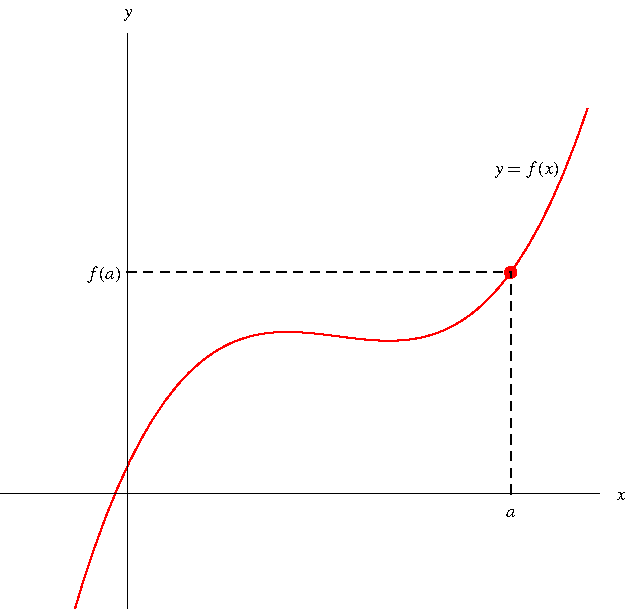
\includegraphics[height=4.5cm]{continuity/pictures/02-05-continuous.pdf}%
\column{.5\textwidth}
\uncover<2->{
The definition requires three things if $f$ is continuous at $a$.
\begin{enumerate}
\item  $f(a)$ is defined (i.e., $a$ is in the domain of $f$).
\item  $\lim_{x\rightarrow a}f(x)$ exists.
\item  $\lim_{x\rightarrow a}f(x) = f(a)$.
\end{enumerate}
}
\end{columns}
\end{frame}
% end module continuous-def
